\documentclass{IEEEtran}
\usepackage{cite}
\usepackage{amsmath,amssymb,amsfonts}
\usepackage{algorithmic}
\usepackage{graphicx}
\usepackage{textcomp}

%Tilføjet packages udover skabelon
\usepackage{graphicx}
\usepackage[table,xcdraw]{xcolor}
\usepackage{pdfpages}
\usepackage{svg}
\usepackage{mathtools}
\usepackage{caption}
\usepackage{subcaption}
\usepackage{blkarray, bigstrut}
\usepackage[backend=biber,
            style=numeric,
            %backref=true,
            abbreviate=false,
            dateabbrev=false,
            alldates=long
            ]{biblatex}

\usepackage{supertabular,booktabs}
\usepackage{multicol}
\usepackage{float}
\usepackage{multirow}
\usepackage{titlesec}


\usepackage{diagbox}

%%%TEST%%%   
\usepackage[per-mode = symbol]{siunitx}   % physical quantities and SI units
%%%%%%%%%%%

\addbibresource{bibliography/Bibliography.bib}


\def\BibTeX{{\rm B\kern-.05em{\sc i\kern-.025em b}\kern-.08em
    T\kern-.1667em\lower.7ex\hbox{E}\kern-.125emX}}

\captionsetup{font=small,labelfont=small, labelfont = bf}

%\captionsetup[figure]{font=footnotesize,labelfont=footnotesize, labelfont = bf}
\begin{document}

\title{A whole-body multi-scale mathematical model for dynamic simulation of the metabolism in man}

\author{Jacob Bendsen, Peter Emil Carstensen, Tobias Kasper Skovborg Ritschel, John Bagterp Jørgensen
\thanks{J. Bendsen, P.E. Carstensen, T.K.S. Ritschel and J.B. J{\o}rgensen are with Department of Applied Mathematics and Computer Science, Technical University of Denmark, Kgs Lyngby, Denmark. Corresponding author: J.B. J{\o}rgensen (e-mail: jbjo@dtu.dk).}
}

\maketitle

\begin{abstract}
We propose a framework to formulate a mathematical model relating cell metabolism to a whole-body flux model. Using this approach we are able to write a large metabolic network generalized by a few compact differential equations. Using qualitative knowledge of biochemical pathways, an example of a model containing 7 organs, 16 metabolites and 31 enzymatic reactions are stipulated to show how this method can be applied to model the metabolism of the three macronutrients carbohydrates, protein and lipids. All reaction rates inside cells are described by Michaelis-Menten kinetics with an addition of a hormonal regulator based on the two hormones insulin and glucagon.  Ingestion of food is added to the model to simulate metabolite concentrations during the fed-fast cycle. The model can simulate over several days while still maintaining physiological relevance due to the inclusion of storage forms that can be depleted if food is not ingested regularly. This is a unique feature compared to similar mathematical models. A physiological model incorporating complex cellular metabolism and whole-body mass dynamics can assist development of therapies and control algorithms for metabolic diseases such as diabetes and obesity.
\end{abstract}

\begin{IEEEkeywords}
Mathematical modeling, metabolism, systems biology, cyber-medical systems, multi-scale modeling, quantitative systems pharmacology

\end{IEEEkeywords}

\section{Introduction}
\label{sec:introduction}





%Behovet for denne type model
%Complex mathematical models exist in today's literature to describe the metabolic reactions in man, although a simple and intuitive framework, in which these advanced mathematical equations can easily be incorporated is not readily available. This type of modelling is specifically useful in PK-PD drug development, such as enzyme inhibitors/activators or hormonal effects. \\ 



%An almost infinite number of reactions happens in the body constantly, many more than ourselves or others include in their models 

%An extreme number of reactions happen in the body. Modeling all reactions mathematically is a challenging task \cite{dash_li_kim_saidel_cabrera_2008,panunzi_pompa_borri_piemonte_gaetano_2020, sorensen_1978, yasemi_jolicoeur_2021}. To model these reactions in a physiologically relevant setting, requires us to look at the system as a whole-body model. A key benefit to looking at the system of metabolic reactions as a whole-body model, is that it allows us to simulate important metabolic concentrations throughout different compartments (organs) under various conditions. The system being affected by various metabolic concentrations of the different organs, such that homeostasis is attempted for all organs, and not just a single compartment. \\


An extreme number of reactions happens in the body, where the formation and breakdown of new metabolites constantly happen to accommodate the different stages that the human body can be in. This metabolism is diverse, and not two people have the same pharmacokinetical parameters, which poses a challenge in PKPD drug development. However, this issue can be met using complex mathematical equations and parameters, that are fitted to a general population. Doing so, can provide an expected concentration of a metabolite in a single organ. It is necessary to realize that not two organs are the same, and such we need to be organ specific in our reactions. To model these reactions in a physiologically relevant setting, requires us to look at the system as a whole-body model. A key benefit to looking at the system of metabolic reactions as a whole-body model, is that it allows us to simulate important metabolic concentrations throughout different compartments (organs) under various conditions. Complex mathematical models exist in today's literature  that describes the metabolic reactions in man\cite{dash_li_kim_saidel_cabrera_2008,panunzi_pompa_borri_piemonte_gaetano_2020, sorensen_1978, yasemi_jolicoeur_2021}, although a simple and intuitive framework, in which these advanced mathematical equations can easily be incorporated is not readily available.


In order to stipulate a whole-body metabolic model, we need to view the model from a top-down perspective. The five key organs included are: Brain, Heart \& Lungs, Liver, Gut, Kidney. Further, Muscle- and Adipose tissue is simplified as a single compartment each and can therefore be considered as an organ, resulting in a total of seven organs.



%If you want a good model, you need a lot of domain specific knowledge.

% \begin{figure}[H]
%     \centering
%     \includegraphics[width=0.8\columnwidth]{Diagrams/Qualitative whole body.png}
%     \caption{Qualitative whole-body model}
%     \label{fig:whole-body}
% \end{figure}





%Skal denne liste egentlig med? Eller er det måske bare nok med den kvalitative model..

% The following metabolic pathways are considered the most important reactions when looking at metabolism in man \cite{miesfeld_mcevoy_2017}.
% \begin{itemize}
%     \item Glycolysis
%     \item Gluconeogenesis
%     \item Glycogenesis and glycogenolysis
%     \item Lipolysis and lipid synthesis
%     \item Transaminase and protein metabolism
%     \item $\beta$ Oxidation and fatty acid synthesis
%     \item Ketogenesis
%     \item Lactate fermentation \& synthesis
%     \item Pyruvate oxidation
%     \item TCA cycle
%     \item Oxidative phosphorylation
% \end{itemize}

% \textbf{TODO}: Skriv noget mere her, herunder beskrive at vi fremlægger en generel metode til at modellere whole-body metabolisme, hvor man selv kan vælge hvad der skal med i modellen, herunder forklare at hele modellen egentlig kun består i at udfylde r-vektorerne.



In these compartments, many different types of cells are present, and in each of these cells a complex and huge metabolic network allows for metabolism of nutrients. In order to gain an understanding of the complex metabolic network, a simplified qualitative model is presented in Fig. \ref{fig:Qualitative_cell}, showing the overall metabolic processes in a given eukaryotic cell.

\begin{figure}[H]
    \centering
    \includegraphics[width=\columnwidth]{Diagrams/Qualitative model.png}
    \caption{Qualitative model for metabolic system, with the follwoing circulating metabolites: amino acids, lactate, glucose, glycerol, triglycerides, free fatty acids and ketone bodies in the top part of the figure.}
    \label{fig:Qualitative_cell}
\end{figure}

% \textbf{TODO}: Beskriv qualititative model

Many reactions are simplified, such that multiple reactions occurs in a single arrow, i.e. glycolysis. It is this qualitative cell-model that we attempt to model in a whole-body simulation to showcase our approach. While it is not the results itself that are interesting, the framework and flexibility of the model is. \\

As we include lipid and protein storage, we can look at the 4 different stages from fed to starvation: 1) postpandrial, 2) postabsorptive, 3) fasting, and 4) starvation. We note that the the metabolite concentrations qualitatively drastically differ in each of these stages. The postprandial phase is generally characterized by a high insulin-to-glucagon ratio, which stimulates the uptake and storage pathways found in liver, muscle and adipose tissue. The post-absorptive state is a catabolic state, in which glycogenolysis and gluconeogenesis is favoured in the liver to maintain blood glucose levels. In this postabsorptive stage we expect to see a stable glucose concentration, with reducing glycogen concentrations \cite{gropper_smith_carr_2018}, due to the post-absorptive metabolism being characterized by a higher glucagon-to-insulin ratio. Fasting is generally defined as 18 to 48 hours after consuming a meal. In this fasting stage, blood glucose concentration begins to fall slowly, as glycogen stores are further depleted, and gluconeogenesis cannot keep the glucose levels constant by itself. The glucagon-to-insulin ratio further increases, facilitating gluconeogenesis. Additionally, amino acid levels are increased as the breakdown of muscle proteins is further facilitated for use in gluconeogenesis. The lipolysis in adipose tissue intensifies to provide fatty acids for fuel and glycerol for gluconeogenesis. When fasting increases beyond 48 hours, it is characterized as starvation. A major shift in metabolic fuels occurs, as the body tries to preserve proteins. Lipolysis rates accelerates, and fatty acids are the main source of energy in most tissues. As the brain can’t utilize fatty acids, ketone bodie formation is substantially increased in the liver. This becomes the main fuel for the brain, as well as being utilized by heart and skeletal muscle for energy. 


Prior to presenting our model, we will first show an example of the mathematical model in a simple scenario, before expanding on all parameters to showcase the whole-body system. 


\section{Mathematical model}
\label{sec:mathmaticalmodel}

% \textbf{TODO}: Beskriv hvad der foregår

The general model can be thought of as a system in which something flows in, its contents get changed, and flows out, defined by the general differential equation

\begin{equation}
\label{eq:general_eq}
    V \frac{dc}{dt} = M (Q_{in}C_{in} - Q_{out}C) + RV
\end{equation}

In which the production rate R, is incorporated as a vector defined by
$C$: concentration of metabolites,
$Q$: tissue specific flowrate,
$M$: external and internal component ordering,
$R$: production rates,
$V$: tissue specific volume,


\begin{equation}
    R = (T S)' T r
\end{equation}
$T$: selection of reactions that occur,
$r$: kinetics for the reactions,
$S$: Stoichiometric matrix containing all reactions.

With the reaction kinetics r, defined as a function of the concentration of each metabolite

\begin{equation}
    r = r(C)
\end{equation}



% \begin{subequations}
% \begin{align}
%     r &= r(c) 
% \\  R &= (T S)' T r 
% \\    \frac{dc}{dt} &= \frac{Q}{V} M \left( c_{in} - c \right) + R
% \end{align}
% \end{subequations}


% Model for each organ
% \begin{equation}
%     V \frac{dc}{dt} = Q (c_{in}-c) + J V
% \end{equation}
% c: blood concentration and only metabolites in blood

% \begin{align}
%     & V \frac{dC_e}{dt} = J V +  R_e V \\
%     & V \frac{d C_i}{dt} = R_i V
% \end{align}


% $C_e = c$: gives $J$ and
% \begin{align}
%     & V \frac{dc}{dt} = Q (c_{in} - c) + R_e V \\
%     & V \frac{dC_i}{dt} = R_i V
% \end{align}


% \begin{equation}
%     R = \begin{bmatrix} R_e \\ R_i \end{bmatrix} = 
%     \begin{bmatrix} S_e' \\ S_i'\end{bmatrix} r = S' r
% \end{equation}

% \begin{equation}
% C = [C_e; C_i] = [c; C_i]
% \end{equation}

%\textbf{TODO}: Notation og illustration af vores model princip er vigtigt. a) single compartment organ, b) two-compartment organ, c) Reactions in cells of organs, d) mass balances, e) stoichiometry and production rates (reaction rates), f) kinetics (enzyme kinetics)

\subsection{Example model}

We now present an example of the model's method and logic, in a simple three compartment model (\textit{k}) with six metabolites (\textit{i}) and six reactions (\textit{j}), resulting in 3 differential equations and stoichiometric matrix 6 by 6. We call this the example model. This results in the following sets:
\begin{align*}
k \in K & =  H,L,G \\
i \in I & =  A, B, C, D, E, F \\
j \in J & =  r_1, r_2, r_3, r_4, r_5, r_6
\end{align*}


\begin{figure}[H]
    \centering
    \includegraphics[width=0.87\columnwidth]{Diagrams/example_diagram_v3.pdf}
    \caption{Schematic representation of the example model. Solid arrows represent blood circulation. $M,C_k,V_k$ represents the blood tissue exchange and $R_k$ represents the reactions happening inside the cell. The dotted lines in the compartments suggests free diffusion, as cell-permeability is not included.}
    \label{fig:example_flow}
\end{figure}

The blood circulation can be split into two parts, the arteries (red) and the veins (blue). The total blood flow, Q, is at all times preserved, and the local blood flow can be calculated using mixers and splitters. They are either explicitly modelled as organs, or implicitly as shown by the triangle (splitter) or square (mixer). A splitter divides the blood flow: $a_1 = a_2 + a_3$, and a mixer combines: $v_2+v_3 = v_1$. The same is true for organs. From the flow diagram, the L-compartment is a mixer so: $v_4+a_2 = v_2$ and the G-compartment is a splitter so: $a_3 = v_4+v_3$. As blood flow is preserved, the flow coming into the H-compartment is the same as the flow coming out of the \textit{H}-compartment. \\

The differential equations describing the mass conservation for each organ are all in the form \eqref{eq:general_eq}.
%When translating to differential equations, each organ is described similarly to (\ref{eq:general_eq}).
% For clarity, we attribute each flow a from and to subscript. This allows us to describe figure \ref{fig:example_flow} by 3 differential equations that describe the mass balance. \\

\begin{subequations}
\begin{align}
    V_H\frac{dC_H}{dt} & = M (Q_{LH} C_L + Q_{GH} C_G - Q_H C_H) + R_H V_H \\
    V_L\frac{dC_L}{dt} & = M (Q_{GL} C_G + Q_L C_H - Q_{LH} C_L) + R_L V_L\\
    V_G\frac{dC_G}{dt} & = M (Q_G C_H - Q_{GL} C_G - Q_{GH} C_G) + R_G V_G
\end{align}
\end{subequations} \\
The subscript Q$_{LH}$ is the blood flow from the liver to the heart. And can be derived as: $Q_{LH} = v_2 = a_2+v_4$. \\


As this model utilizes a stoichiometric matrix to model cell metabolism \cite{yasemi_jolicoeur_2021} we include the addition of $M$ and R$_k$. $M$ is a square matrix only containing ones and zeros in the diagonal corresponding to the circulating metabolites. In this example A and D are the circulating metabolites. R$_k$ is the production rates of metabolites inside the tissues. 
The reactions occurring inside the each of the compartments in Fig. \ref{fig:example_flow} is described by Fig. \ref{fig:example_metabolic_map} and Table \ref{tab:example_stoichio_table} \\

\setlength\extrarowheight{-4pt}
\begin{table}[H]
\centering
 \caption{Summary of the stoichiometric reactions and its kinetics in the example model.}
 \label{tab:example_stoichio_table}
 \resizebox{0.75\columnwidth}{!}{
  \begin{tabular}{*{3}{c}}
   %\toprule
    \# R  & Stoichiometric   & Kinetic \\[0.5ex]
   \midrule
    1 &  $A \rightarrow F$  &  $r_1 = p_1 C_A$  \\
   \midrule
    2 &  $F \rightarrow A$  &  $r_2 = p_2 C_F$ \\
   \midrule
    3 &  $F \rightarrow C$  &  $r_3 = p_3 C_F $  \\
   \midrule
    4 &  $A + C \rightarrow B$  &  $r_4 = p_4 C_A C_C$ \\
    \midrule
    5 &  $B \rightarrow D$  &  $r_5 = p_5 C_B$  \\
    \midrule
    6 &  $D \rightarrow E$  &  $r_6 = p_6 C_D$  \\
   \bottomrule
  \end{tabular}
  }
\end{table}

\setlength\extrarowheight{0pt}

$r$ is a reaction rate, that depends on the concentration $C$ and a scalar $p$.
% $r$: reaction rate,
% $p$: scalar. \\



To calculate R$_k$ in the three equations, the stoichiometric matrix is defined based on table \ref{tab:example_stoichio_table}  \\


%\textbf{TODO}: Further description of example


% \textbf{TODO}: Find en god måde at referere til "Modelling Cell Metabolism: A Review on Constraint-Based Steady-State and Kinetic Approaches" \cite{yasemi_jolicoeur_2021}


\begin{equation}
\label{eq:stoi_example}
S =
\begin{blockarray}{l c c c c c c}
\begin{block}{l c c c c c c}
& A & B & C & D & E & F & \\
\end{block}
\begin{block}{l [c c c c c c]}
r_1 & -1 & 0  & 0  & 0  & 0 & 1 \\
r_2 & 1  & 0  & 0  & 0  & 0 & -1 \\
r_3 & 0  & 0  & 1  & 0  & 0 & -1 \\
r_4 & -1 & 1  & -1 & 0  & 0 &  0 \\
r_5 & 0  & -1 & 0  & 1  & 0 & 0 \\
r_6 & 0  & 0  & 0  & -1 & 1 & 0 \\
\end{block}
\end{blockarray}
\end{equation}

%Where each row describes which reactions take place, 

Where each row contains the stoichiometric coefficients of each reaction, in each compartment described by the columns. To find the changes in concentrations in each compartment we must define a compartment specific matrix, that defines which reactions happens in each cell. To do this we use $T_k$. In this example we define $T_H$ in the \textit{H}-compartment where only universal reactions 1, 2 and 6 occurs.


\begin{equation}
    T_H = 
    \begin{bmatrix}
        1 & 0 & 0 & 0 & 0 & 0 \\
        0 & 1 & 0 & 0 & 0 & 0 \\
        0 & 0 & 0 & 0 & 0 & 1
    \end{bmatrix}
\end{equation}

In doing so we can then find the changes in the production rate of the \textit{H}-compartment vector $R_H$ as

 
\begin{equation}
    R_H =  (T_HS)'T_Hr_H 
    %    = \begin{bmatrix}
    %     -r_1 + r_6 \\
    %     r_1 - r_6 \\
    %     -r_6 \\
    %     -r_1 + r_2 \\
    %     -r_2 \\
    %     0
    % \end{bmatrix}
\end{equation}

%The metabolic pathways in our example is illustrated in figure \ref{fig:example_metabolic_map}.

\begin{figure}[H]
    \centering
    \includegraphics[width=0.8\columnwidth]{Diagrams/example_cell.pdf}
    \caption{Diagram of metabolic pathways in cell. The hollow double-sided arrows means the metabolite is distributed through the blood. The black arrows indicate reactions that happen in all compartments. The grey arrows indicate reactions that happen in some compartments. Reactions are numbered corresponding to the stoichiometric matrix (\ref{eq:stoi_example}).}
    \label{fig:example_metabolic_map}
\end{figure}


Each reactions kinetic can be described dependant on the reactant being used and an equation describing enzyme kinetics. These equations could e.g. be Hill equations or Michaelis-Menten kinetics. Further several additions could be made here to include reaction specific equations, such as hormonal effect, or capacity-limited reactions. \\

While cell-permeability is not included in this example, it could be represented in the compartments, as one could include a vascular and interstitial compartment, where only circulating metabolites are exchanged between the two compartment, resulting in an increased delay.



%\vfill\eject
\newpage
\subsection{Model}

% \textbf{TODO}: Måske lidt mere introduktions tekst her? fx sige at vi har brugt den fremlagte metode til at udforme netop denne model.
% Formål med denne model?

We now present a model containing 7 compartments and 16 metabolites split into 31 reactions including hormonal effect from the two signal molecules, insulin and glucagon, on specific tissues. We create the model using the same methodology as described earlier. The purpose is to describe the energy metabolism of the three macronutrients protein, carbohydrates and lipids. We include the major biochemical pathways which these macronutrients are a part of, in order to simulate their behaviour under various conditions. The two hormones are included to add stability and avoid large transient periods in the simulation after intake of food, as insulin and glucagon are important anabolic and catabolic hormones respectively. \\


\begin{figure}[H]
    \centering
    \includegraphics[width=0.82\columnwidth, keepaspectratio]{Diagrams/Bendsen_Carstensen_Flow_v4.pdf}
    \caption{Schematic representation of the whole-body model. Solid arrows represent blood circulation, where the right side is the arteries and the left side the veins.
    Thick arrows, $a_2$ and $v_2$, represents joining of flows from other organs.
    $M$,$C_k$,$V_k$ represents the blood tissue exchange and $R_k$ represents the reactions happening inside the cell. The dotted lines in the compartments suggest free diffusion, as cell-permeability is not included.}
    \label{fig:Bends_cars_flow_diagram}
\end{figure}


\begin{figure}[H]
    \centering
    \includegraphics[width=\columnwidth]{Diagrams/Metabolic_map_artikel_v3_numeric.pdf}
    \caption{Diagram of metabolic pathways in cell. The hollow double-sided arrows means the metabolite is distributed through the blood. The black arrows indicate reactions that happen in all organs. The grey arrows indicate reactions that only happen in some organs. Metabolites are shown as 2-4 letter abbreviations. Reactions are numbered corresponding to the stoichiometric matrix.}
    \label{fig:metabolic_map}
\end{figure}

From figure \ref{fig:metabolic_map} it follows, that many pathways are cell specific. 10 of 31 reactions occurs in all organs. The remaining 21 are tissue specific, as the different organs each have a specialized role. Insulin and glucagon secretion/clearance is incorporated as a single reaction for simplicity, as they are not created by nor metabolised into any included metabolite. Their production rates are inherited from Sorensen \cite{sorensen_1978}, as described in section \ref{sec:hormonal_model}.\\

The most accurate mathematical equations to describe each of these 31 metabolic reactions, is not necessarily known, and varies from individual to individual. This means that each of these reactions has be simplified. In our model, We describe the reaction rates using Michaelis-Menten kinetics which may or may not be an overly simplistic description of the actual reactions. To change the systems dynamics, you can simply modify the mathematical formula in the reaction rate vector. Michaelis-Menten is especially useful for describing enzyme reactions, as enzyme reactions have an upper limit to how fast they can occur. Although this type of kinetics is not the only type that can be included, it is possible to change these to other functions, such as positive hyperbolic tangent functions \cite{sorensen_1978} or simple first-order kinetics \cite{kim_saidel_cabrera_2006}\\


\vfill\eject


\begin{table}[H]
    \centering
    \caption{Summary of metabolic pathways in all tissues. Organs are in the columns and reactions in the rows. Grey squares means the reaction is present in the organ, white squares means the reaction is disregarded. The reactions can be found according to their number in appendix \ref{tab:appendix_reaction}}
    \label{tab:summary_pathways}
    \includegraphics[width=\columnwidth]{Diagrams/artikel_tabel_II.pdf}
\end{table}

Table \ref{tab:summary_pathways} summarizes what reactions are included in what organs in the model. If a reaction is excluded from an organ, it does not mean that the reaction never happens in reality. It instead means that the reaction is not significant enough to include for our simplified model. An example is glycogen formation that also happens in brain, heart and adipose tissue, but it is in such small quantities, that it becomes negligible. \\




\subsection{Inclusion of a hormonal model}
\label{sec:hormonal_model}

% \textbf{TODO}: Omskrives fra bachelor \\

% \textbf{TODO}: Læs igennem og ret 

Different implementations of hormonal models are possible and available, however Sorensen \cite{sorensen_1978} employs a very simple Glucagon model that describes pancreatic glucagon release. Sorensen found that the glucagon release and clearance could be described adequately by a one compartment model. Sorensen also formulated an insulin model described by a six compartment model. The models are a product of comparing literature and experimental data.
While it is possible to include the glucagon model as a single compartment model and insulin in a 6 compartment model, similar to \cite{panunzi_pompa_borri_piemonte_gaetano_2020,sorensen_1978}, it would be best practice to include insulin and glucagon in a whole-body 7 compartment model, to ensure a single methodology. Insulin and glucagon are therefore included in the stoichiometric matrix as metabolites in order to calculate their production rates. \\

To represent the effect that the hormones insulin and glucagon have on organ specific reactions, we now list a table containing which reactions are affected by insulin and glucagon, as well as in which organ. \\


%\begin{tabular}[c]{}{} Liver, muscle tissue \\ adipose tissue \end{tabular}
\setlength\extrarowheight{2pt}
\begin{table}[H]
\centering
 \caption{The following reaction are affected by insulin and glucagon \cite{ gropper_smith_carr_2018, miesfeld_mcevoy_2017}.
$\Uparrow$, symbolizes increased stimulation, $\Downarrow$, symbolizes decreased stimulation. Table is sorted by effect.}
 \label{tab:insulin_glucagon_reactions}
 \resizebox{\columnwidth}{!}{
  \begin{tabular}{lcccc}
   %\toprule
    \textbf{Hormone} & \textbf{\# R} & \textbf{Reaction} & \textbf{Effect} & \textbf{Affected Organs} \\[0.5ex] \hline
    \textbf{Insulin}  & 1 & GLC $\rightarrow$ G6P & $\Uparrow$ &  Liver, muscle tissue, adipose tissue \\ \cmidrule{2-5}
    & 3 & G6P $\rightarrow$ 2GA3P & $\Uparrow$ & Liver, muscle tissue \\ \cmidrule{2-5} 
    & 5  & G6P $\rightarrow$ GLY & $\Uparrow$ & Liver, muscle tissue \\ \cmidrule{2-5} 
    & 13 & PYR $\rightarrow$ ACoA & $\Uparrow$ & Liver, muscle tissue \\ \cmidrule{2-5} 
    & 21 & TGL $\rightarrow$ 3FFA + GLR & $\Uparrow$ & Adipose tissue \\ \cmidrule{2-5} 
    & 23 & 7ACoA $\rightarrow$ FFA & $\Uparrow$ & Liver \\ \cmidrule{2-5} 
    & 26 & AA $\rightarrow$ PRO & $\Uparrow$   & Muscle tissue \\ \cmidrule{2-5} 
    & 28 & 3FFA + GLR $\rightarrow$ TGL_{AP} & $\Uparrow$   & Adipose tissue \\ \cmidrule{2-5} 
    & 4 & 2GA3P $\rightarrow$ G6P & $\Downarrow$  & Liver \\ \cmidrule{2-5} 
    & 6 & GLY $\rightarrow$ G6P & $\Downarrow$    & Liver, muscle tissue \\ \cmidrule{2-5}
    & 27 & PRO $\rightarrow$ AA & $\Downarrow$    & Muscle tissue           \\ \cmidrule{2-5}
    & 29 & TGL_{AP} $\rightarrow$ 3FFA + GLR & $\Downarrow$     & Adipose tissue \\ 
    \midrule 
    \textbf{Glucagon} & 4 & 2GA3P $\rightarrow$ G6P & $\Uparrow$ & Liver \\ \cmidrule{2-5} 
    & 6 & GLY $\rightarrow$ G6P & $\Uparrow$ & Liver \\ \cmidrule{2-5} 
    & 29 & TGL_{AP} $\rightarrow$ 3FFA + GLR & $\Uparrow$ & Adipose tissue \\ \cmidrule{2-5} 
    & 3 & G6P $\rightarrow$ 2GA3P & $\Downarrow$ & Liver \\ \cmidrule{2-5}
    & 5 & G6P $\rightarrow$ GLY & $\Downarrow$ & Liver \\  
   \bottomrule
  \end{tabular}
  }
\end{table}
\setlength\extrarowheight{0pt}

% Similar models, \cite{dash_li_kim_saidel_cabrera_2008,sorensen_1978,panunzi_pompa_borri_piemonte_gaetano_2020}, has had actual data to parameter-estimate over, allowing an increased complexity, to utilize functions similar to 
% \begin{equation}
%     \mu_1 + \mu_2\cdot tanh\left(\mu_3\cdot\left(\frac{I}{I^B} - \mu_4\right)\right)
% \end{equation}
% Where a total of four $\mu$ parameters needs to be parameter-estimated. $B$ indicates steady-state value. 

While the qualitative effect of insulin and glucagon is known, explicitly in table \ref{tab:insulin_glucagon_reactions}, the mathematical impact that insulin and glucagon has, is not necessarily known. We only know, from literature, which enzymes and hence reactions they have an effect on. We use a simple function where, given the reciprocal effects of insulin and glucagon, the ratio between these two hormones allows us to determine whether or not they have an effect on the system. These functions alter the production rates of the reactions in table \ref{tab:insulin_glucagon_reactions}:
\begin{equation}
    \textbf{Insulin activation}: \left(\frac{I_k}{I_k^B}\right)^{\mu_j}\cdot V_{max_j}
\end{equation}
\begin{equation}
    \textbf{Insulin inhibition}: \left(\frac{I_k^B}{I_k}\right)^{\mu_j}\cdot V_{max_j}
\end{equation}
And if both insulin and glucagon have an effect on the same reaction (though opposite effects), the insulin-to-glucagon or glucagon-to-insulin ratio is instead used:
\begin{equation}
    \textbf{Insulin-to-Glucagon stimulation}: \left(\frac{\Gamma_k^B}{\Gamma_k}\cdot \frac{I_k}{I_k^B}\right)^{\mu_j}\cdot V_{max_j}
\end{equation}
\begin{equation}
    \textbf{Glucagon-to-insulin stimulation}: \left(\frac{\Gamma_k}{\Gamma_k^B}\cdot \frac{I_k^B}{I_k}\right)^{\mu_j}\cdot V_{max_j}
\end{equation}

Where $j$ is the reaction, fx GLC$\rightarrow$G6P, $k$ is the compartment and the superscript $B$ indicates the basal-value. These simple functions are equal to 1 at steady state, which occurs when blood glucose is at 5mM, which means that no matter the value of $\mu$, the effect is not present at steady-state. This is a very important property, since many of the parameters used in the reactions are estimated based on metabolite homeostasis. \\


%have the property of being equal to 1, no matter the size of $\mu$. if the insulin and glucagon ratios are equal to 1, which they are at steady state when blood glucose = 5mM. This is a very important property, since many of the parameters used in the reactions are estimated based on metabolite homeostasis. \\

\subsection{Inclusion of a modified SIMO-model}  

% \textbf{TODO}: Læs igennem og ret 

A modified version of the Simple Interdependent glucose/insulin MOdel, SIMO, \cite{panunzi_pompa_borri_piemonte_gaetano_2020} is used to include the uptake of glucose, amino acids and fats from ones diet. The rates are the same for all macronutrients, which is not physiologically true, as these macronutrients differ in terms of absorption given their molecular differences, but in lack of data or other mathematical models describing this issue, the SIMO model is the best and simplest choice. \\

\begin{figure}[H]
    \centering
    \includegraphics[width=0.75\columnwidth]{Diagrams/SIMO.pdf}
    \caption{Schematic representation of digestive tract. SIMO \cite{panunzi_pompa_borri_piemonte_gaetano_2020}, S represents the amount of macronutrients in the stomach, J the jejunum which is the first part of the small intestine, R a delay and L the amount in ileum which is the second part of the small intestine. $r_{oga}$ is a vector describing the uptake of the 3 macronutrients}
    \label{fig:simo}
\end{figure}

% In the equations used in the model the compartments S, J, R and L are all 3x1 vectors: \\
% \begin{equation}
%     \begin{split}
%         \dot{S}  = \begin{bmatrix}
%               S_{GLC} \\
%               S_{AA} \\
%               S_{TGL}
%              \end{bmatrix},
%              \dot{J}  = \begin{bmatrix}
%               J_{GLC} \\
%               J_{AA} \\
%               J_{TGL}
%              \end{bmatrix} \\
%              \dot{R}  = \begin{bmatrix}
%               R_{GLC} \\
%               R_{AA} \\
%               R_{TGL}
%              \end{bmatrix},
%              \dot{L}  = \begin{bmatrix}
%               L_{GLC} \\
%               L_{AA} \\
%               L_{TGL}
%              \end{bmatrix}
%     \end{split}
% \end{equation}

The resulting uptake of nutrients is represented by the equation:
\begin{equation}
    r_{oga} = k_{gj}J + k_{gl}L = \begin{bmatrix}
           k_{gj}J_{GLC} + k_{gl}L_{GLC} \\
           k_{gj}J_{AA} + k_{gl}L_{AA} \\
           k_{gj}J_{TGL} + k_{gl}L_{TGL}
         \end{bmatrix}
\end{equation}

$r_{oga}$ is a 3$\times$1 vector, where the first two macronutrients, i.e. glucose and amino acids, are taken up by the gut. This is not the case for triglycerides, which enters the lymphatic system as chylomicrons and is transported to muscle and adipose tissue before it enters the blood circulation\cite{gropper_smith_carr_2018}. The last instance of $r_{oga}$ is then delivered to muscle and adipose tissue, where a 50/50\% distribution is assumed in the two tissues. As the specific uptake rate of amino acids and fat is not explicitly known from the SIMO model, we utilize the uptake rate $k_{gj}$ and $k_{gl}$ from glucose.\\

It is then included in the model as the parameters:
\begin{center}
    Gut: $G_{r_{oga}}$ \\
    Muscle: $MP_{r_{oga}}$ \\
    Adipose: $AP_{r_{oga}}$
\end{center}

The modified SIMO model is included as additional inputs in the differential equations and not directly into the production rate vector R. This is done as the SIMO model provides external inputs from meal consumption and thought of as an extension to the general methodology.


% To summarize \\
% $G_{r_{oga}}$ transports glucose and aminoacids to the gut\\
% $MP_{r_{oga}}$ transports triglycerides to muscle tissue \\
% $AP_{r_{oga}}$ transports triglycerides to adipose tissue \\


%\textbf{TODO}: Beskriv at det naturligvis ikke er retfærdigt at optagelsesraterne er ens for GLC, AA og TGL





In section II.B through section II.D all constitute to create a single larger model. This will be referenced in the following sections as 'the model'.


\section{Simulation results}
\label{sec:simulationresults}

We now simulate the model in MATLAB. Initially we present the model with a single initial meal ingested at steady-state, and following the development of metabolites as the 25 year old in silico patient refrains from eating or doing physical activity for the next 72 hours. \\


%Indsæt simulerings resultater
% \textbf{TODO}: Disse simulerings resultater bør køres med Fed/Fast stages. Samt skal y-aksen gøres nice og muligvis udelade nogle af dem. Glycogen er vigtig at have med.


% \textbf{TODO}: Beskriv 4 forskellige stadier



\begin{figure}[H]
    \centering
    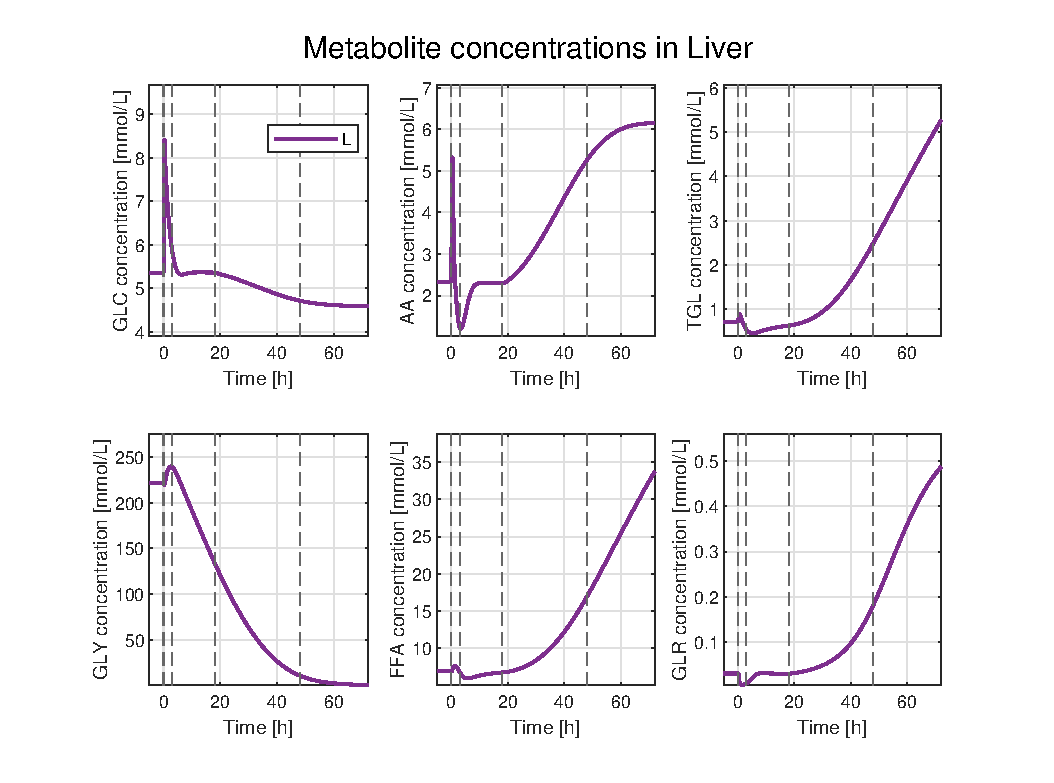
\includegraphics[trim=35 10 35 0, width=\columnwidth]{Diagrams/Fasting/liver_metabolites.eps}
    \caption{Metabolite concentrations in the liver after an initial meal of 60g glucose, 24g protein and 16g fat and an accompanying fast for 72 hours, in the model.}
    \label{fig:Liver_metabolites}
\end{figure}

Figure \ref{fig:Liver_metabolites} shows glucose, amino acids, triglycerides, glycerol, free fatty acids and glycogen. The first 3 plots shows the metabolites that are ingested through the SIMO model. During fasting after an initial meal, we see that glucose initially rises, and then returns to the baseline where it plateaus for roughly 24 hours, after which it starts to drop. This drop happens at about the same time as glycogen in the liver goes towards 0. It is shortly after this drop in glucose that the concentration of certain other metabolites start increasing, especially the glycerol, free fatty acid and triglyceride metabolites as it enters the starvation stage. An increase in triglycerides is seen during starvation as the triglyceride storage in the adipose tissue, TGL$_{AP}$, concentration drops. Free fatty acids levels increasing substantially during starvation is to be expected based on articles that investigates the effects of starvation \cite{unger_eisentraut_madison_1963, yaffe_1980A}.
brain, as well as being utilized by heart and skeletal muscle.\\

\subsection{Fluxes inside the cells}

While it is important to keep in mind that these simulation results are not physiologically accurate for all metabolites, we can plot the fluxes in order to help us highlight the dynamics.


% \textbf{TODO:} Why are flux plots interesting to simulate / hvad er det vi ser / beskrivelse af hver organs rolle, ie. lever producerer hjerne forbruger

\begin{figure}[H]
     \centering
     \begin{subfigure}{1\columnwidth}
         \centering
         \caption{}
         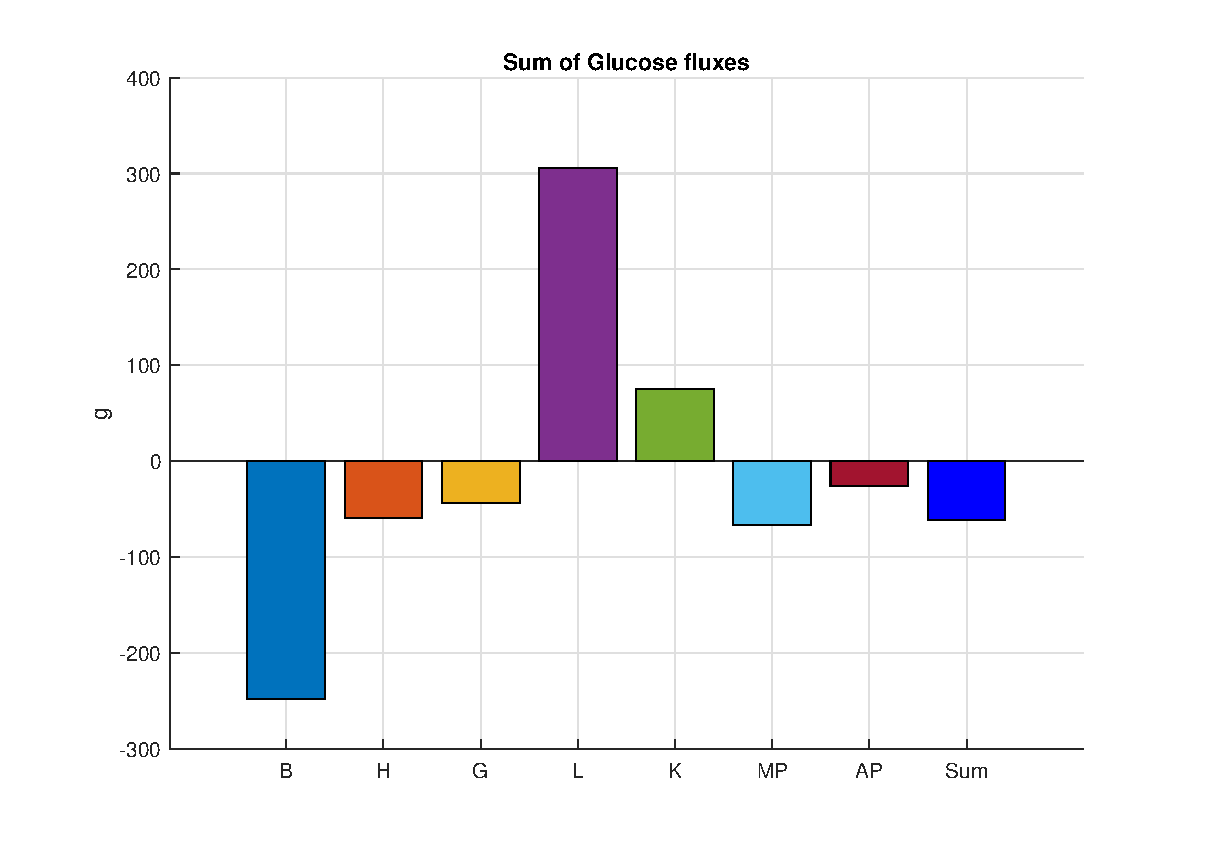
\includegraphics[width=\columnwidth]{Diagrams/Fasting/Flux/bar_plot_flux.eps}
         \label{fig:barplot_glucose}
     \end{subfigure}
     \hfill
     \begin{subfigure}{1\columnwidth}
         \centering
         \caption{}
         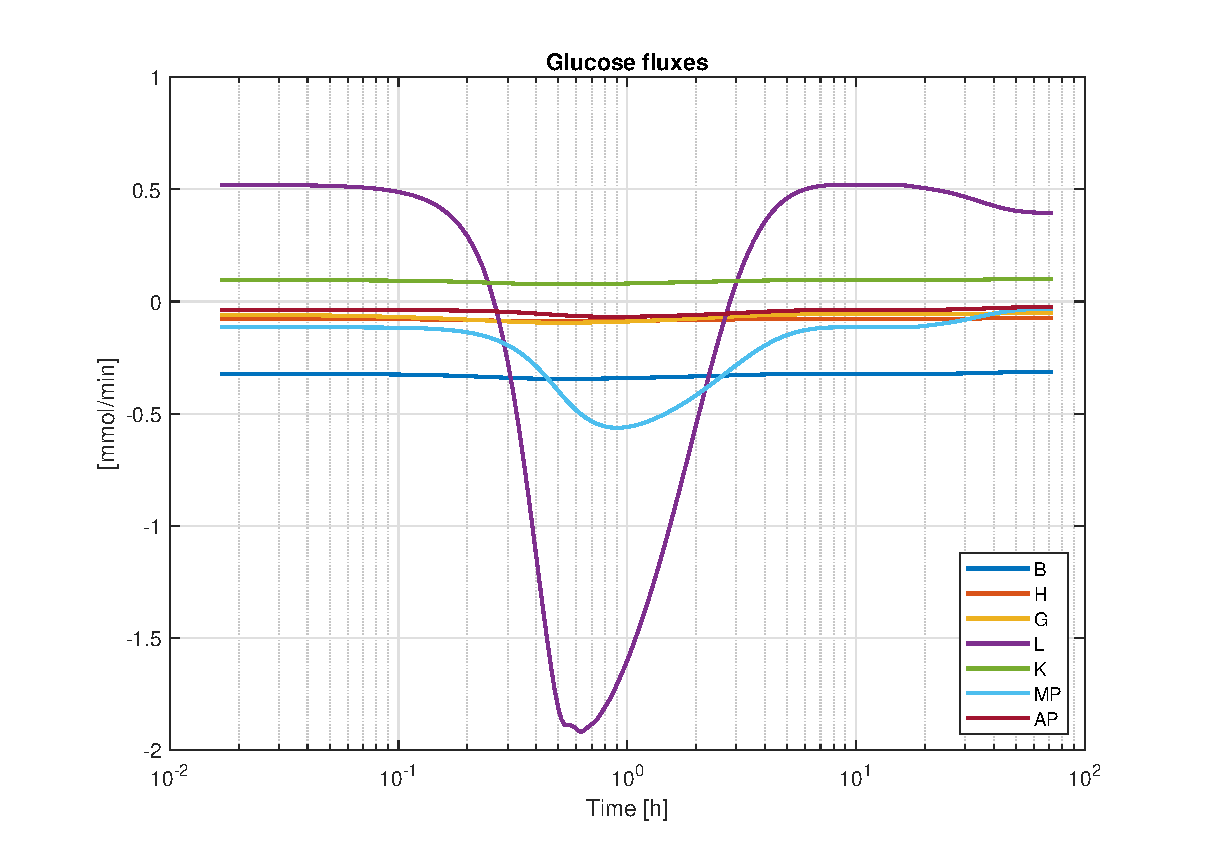
\includegraphics[width=\columnwidth]{Diagrams/Fasting/Flux/glucose_flux.eps}
         \label{fig:glucose_flux_plot}
     \end{subfigure}
     \caption[short]{Brain and heart flux, in the model, after an initial meal and accompanying fasting for 72 hours. (a) Shows the cumulative fluxes of the organs. (b) Shows fluxes during the time period with a logarithmic scale on the x-axis.}
    \label{fig:glucose_flux}
\end{figure}



% \textbf{TODO}: Vigtigste simulationsresultater: Flux og normale plots til at beskrive fed-fast cycle + noget der kan vise hormonregulering og hvordan den fungerer. Til at vise hormon regulering, skal man vise med og uden hormon regulering i ét plot? 

We see that in figure \ref{fig:glucose_flux}a, the brain is a major consumer of glucose, and the liver is a major exporter of glucose  \cite{miesfeld_mcevoy_2017}. The sum shows the net flux of glucose in all organs, resulting in an overall consumption corresponding to a meal containing 60g glucose. Quite interestingly figure \ref{fig:glucose_flux}b shows which organs are the consumers of glucose over log time. There is a large drop initially for the glucose flux in liver and muscle tissue as food is ingested and the blood glucose concentration is high. This is especially seen in the insulin stimulated tissues, as the effect described in table \ref{tab:insulin_glucagon_reactions} shows an increase in glucose uptake as a result of high concentrations of insulin. As the blood glucose concentration reduces, the liver again starts producing glucose for the other organs in order to keep homeostasis and thus increasing its flux to a positive value.


\subsection{Regular food intake}
We now introduce several meals to the system, to simulate a healthy 25 year old male at rest for 72 hours with the macronutrient distribution: \\
\begin{equation*}
\begin{split}
    \text{Carbohydrate}: 60 g \\
    \text{Protein}: 24 g \\
    \text{Fat}: 16 g \\ \hline
    \text{Total}: 100g
\end{split}
\end{equation*}


\begin{figure}[H]
    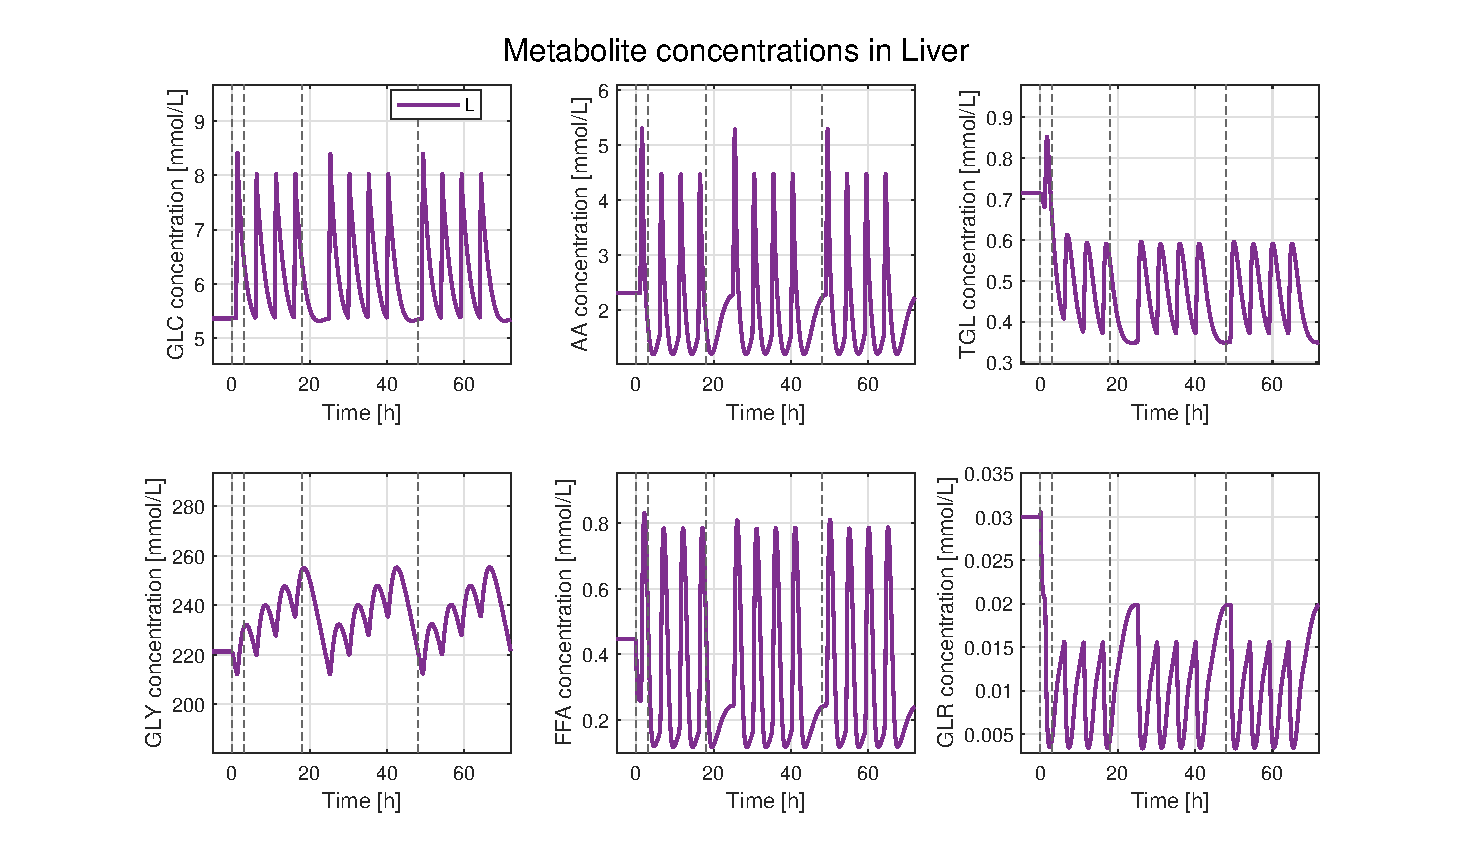
\includegraphics[trim=35 10 35 0, width=\columnwidth]{Diagrams/Food/liver_plot.eps}
    \caption{Metabolite concentrations in the liver after regular meals four times a day with five hours in between and then followed by nine hours of fasting during the night. Simulated over 3 days.}
    \label{fig:food_plots_bends_cars}
\end{figure}


% \textbf{TODO}: Beskriv food plots


In figure \ref{fig:food_plots_bends_cars} each spike corresponds to an intake of food, and we see that eating 4-5 times a day maintains a favourable concentration but with larger spikes. Simulating with smaller meals with increased frequency gives smaller spikes and therefore a more stable concentration for glucose and other metabolites over time \cite{derendorf_schmidt_rowland_tozer_2020}. Looking at the SIMO-model, the concentration of macronutrients in the stomach and ileum is almost depleted. If the food intake is reduced to smaller meals every 2 hours, with a 9 hour break to simulate sleep, a more consistent glucose concentration is seen, as the stomach concentration does not go towards 0, but rather attempts to stabilize and therefore can create a scenario more similar to a constant infusion of food, thus reducing the size of the spikes. The metabolites TGL, GLR and FFA are mostly stable during regular food intake, however, they fall after food intake, as a result of an increase in insulin. This results in increased TGL uptake in adipose tissue as well as increased lipid droplet formation.


\subsection{Specific dieting}

It is possible to suggest different diets, that are effective mathematically. We now present a simulation in which we plot for 13 days, with food intake regularly for 1 day, with 4 meals a day, followed by 9 hours of rest and 24 hours of fasting, resulting in intermittent 24 hour fasting. 

\begin{figure}[H]
    \centering
    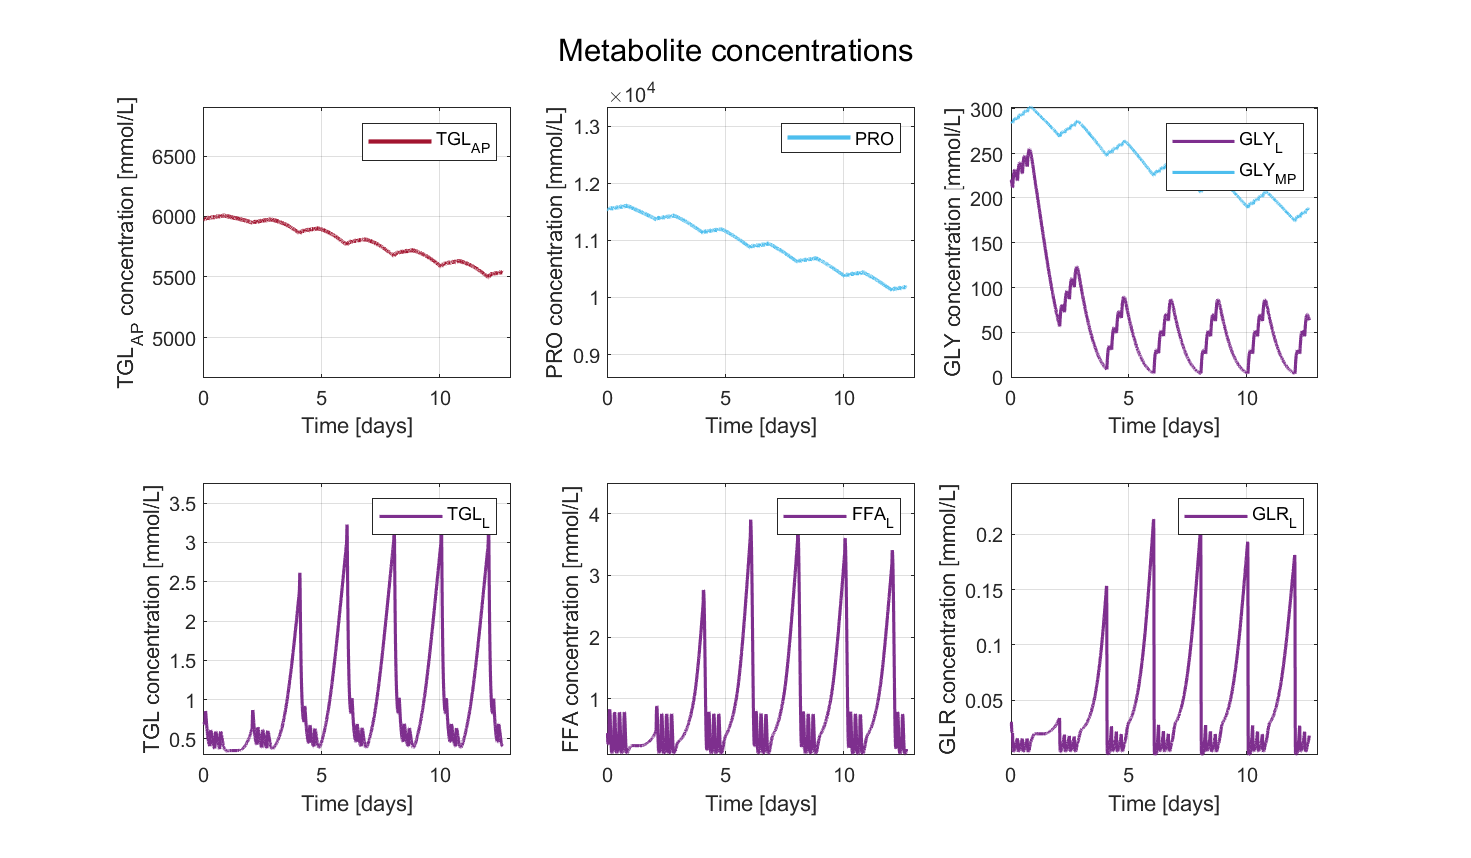
\includegraphics[trim=40 10 40 0, width=\columnwidth] {Diagrams/Food/metabolites_13_days_no_food_33_hours.eps}
    \caption{Storage and fat metabolites during 24 hour intermittent fasting}
    \label{fig:my_label}
\end{figure}

During this intermittent fasting, we expect to see a reduction in the lipid droplet concentration due to the energy balance of this system becoming skewed from a roughly equal kcal intake/consumption, to a 50\% reduction in kcal intake. We see a drop in the concentration of lipid droplets, as they get metabolized into different metabolites to provide energy for the body. Further, we see that the muscle tissue is also broken down, as food becomes a relatively scarce source for the body. Within a day we see a large drop in the concentration of glycogen after the last meal. Glycogen is used initially as an energy storage, but gets depleted quickly in the liver \cite{miesfeld_mcevoy_2017}. The glycogen in the muscle tissue is slowly depleted as the in silico patient is at rest for the entire simulation. The lipid droplets are converted into TGL, FFA and GLR and utilized in different compartments. We see large spikes as the body enters the starvation phase after 18 hours of no food, much like we saw before in figure \ref{fig:Liver_metabolites}. With this intermittent fasting, we are able to show both the effects of regular meal intakes and starvation. \\

\section{Discussion}

\subsection{Assumptions \& Drawbacks}

% \textbf{TODO}: Hvilke assumptions laver vi for at få modellen til at kunne køre. Skrives rent. \\
% Flere assumptions der måske skal beskrives: Er de metabolitter vi har valgt tilstrækkelige eller for komplekse? Er det nok bare med en form for kinetik? 

% Coenzymer, NADH, NAD+, ATP, ADP er ikke medtaget

% Insulin Glucagon model påvirkning er OK nok til at modellere systemet? Er det nok med to signalstoffer? \\


Assumption: Diffusion across cell membranes happens infinitely fast, as the time it takes for the cell to be in equilibrium with the blood vessels happens, at a much faster timescale compared to the timescale of our model. This assumption makes it possible to include organs as one compartment. If transporters and diffusion were to be incorporated in the model, it would be expected to divide the compartments in two, so that transporters could be explicitly modeled.\\

Assumption: The concentration is the same across the entire cell. We model each organ as a well-stirred tank, so every metabolite is uniformly distributed in the organs. It is known that the enzymatic reactions in each cell and organ happens at a rapid timescale of $10^{-3} \text{ to } 10^0$ seconds \cite{yasemi_jolicoeur_2021}. Given the models timescale of hours, up to several days, it can be assumed that the enzymatic reactions happen at a uniform rate across the spatial organs, allowing a simplification of complex enzymatic reactions to be reduced to Michaelis-Menten kinetics. \\

% \textbf{TODO}: Omskrive nedenstående afsnit som "additional work" istedet. \\



It could be theorized that given the introduction of more metabolic inputs, that a model like this could be used to gain a better understanding of the dynamical changes in metabolite concentrations of an individual. Both a generalized model could be used, or one tailored to the specific individuals parameters, thus introducing personalized modelling behaviour. If one would wish to simulate various diseases in enzyme defects, this could be done with the current format of the model, though it would require validation of the model for it to be relevant. \\

Something that would be interesting to incorporate into the model, is the energy balance of the cell. Despite being a significant factor in determining which way the metabolic pathways will go, it was excluded for simplicity. Future work on the model should include adding energy balance to the cell, possibly also including the addition of CO$_2$ and O$_2$ as can be seen other muscle models \cite{dash_li_kim_saidel_cabrera_2008}. The possibilities are there, but it may require in vivo experiments and a more thorough parameter-estimation process.

\section{Conclusion}
\label{sec:conclusion}
% \textbf{TODO}: Skal der noget angående vores eksempel med i konklusionen? \\
% \textbf{TODO}: Mere fokus på metoden istedet for at fokusere på netop den model vi valgte at lave udfra metoden! \\


Through linear algebra and differential equations, we have stated a model that is capable of simulating the complex human metabolism. Our method makes it simple to expand the system to whatever one would like to model, through changes in the stoichiometric matrix that matches the chemistry. Using this approach, the core of the model is simply which parameters and reaction kinetics are used in the production vector R$_k$. This is illustrated in our expanded system, which involves 16 metabolites and 2 hormones in 7 organs. This results in a total of 126 differential equations. The complex system can be written as only 7 differential equations, one for each organ, as the entire reaction network is included in the production rate vector R. \\

As shown, the model framework can easily be expanded to incorporate complex metabolic reactions in man, interestingly, the models framework is applicable to not just a physiological model, but can easily be made to fit chemical systems, with containers, tubes and chemical reactions taking place, or other similar systems, simply by changing the values in the variables, while maintaining the overall framework. \\

The modelling objective was to create the basis for a physiological whole-body model that can incorporate cellular metabolic processes, and as such we hope that this article can give some insight as to how the complex systems in the human body can be explained quantitatively.



% By applying knowledge from Sorensen \cite{sorensen_1978} onto the model which have drawn much inspiration from Kim Cabreras muscle model \cite{dash_li_kim_saidel_cabrera_2008} and biological text books \cite{gropper_smith_carr_2018, miesfeld_mcevoy_2017, vanputte_regan_russo_2019}, we were able to stipulate a model which had many elements of the complex human metabolism. 

% The purpose of this model, was not to stipulate a model which could 

% The purpose of the model was from the start clear, we could not achieve high levels of physiological relevance with limited data, but we were able to formulate a model to quantitatively simulate the biochemical processes in man based on qualitative research.\\

\printbibliography






\onecolumn
\appendix
\setcounter{equation}{0}
\setcounter{table}{0}
\label{sec:appendix}
\renewcommand{\theequation}{\thesection.\arabic{equation}}
\renewcommand{\thetable}{\thesection.\Roman{table}}

\subsection{Model equations}


\begin{table}[H]
\centering
\resizebox{0.8\textwidth}{!}{%
\begin{tabular}{rllrl}
{  \textbf{Variables}} &                 &  & {  \textbf{Subscript}} &               \\
\textbf{C:}    & Metabolite Concentration ($\frac{mmol}{L}$)    &  & \textbf{B:}               & Brain  \\
\textbf{V:}               & Volume ($L$) &  & {  \textbf{G:}}         & Gut \\
\textbf{Q:}    & Vascular plasma flow rate ($\frac{L}{min}$)    &  &\textbf{H:}               & Heart and lungs \\
\textbf{t:}               & Time ($min$)    &  & \textbf{L:}               & Liver \\
\textbf{V$_{max}$:} & Maximum velocity ($\frac{mmol}{min}$)    &  & \textbf{K:}               & Kidney        \\
\textbf{K$_m$:}  & Limiting velocity ($\frac{mmol}{L}$)               &  & \textbf{AP:}              & Adipose   \\
\textbf{M:}  & Circulating metabolites  &  &  \textbf{MP:}            & Muscle \\
{  \textbf{Other}} &                 &  & {  \textbf{}}           &               \\
%\textbf{$p_\phi$:}           & Stoichiometric Matrix          &  & {  \textbf{}}           &               \\
\textbf{R:}                  & Production rates             &  & {  \textbf{}}       
& \\
\textbf{r$_{oga}$:}                  & Nutrient uptake            &  & {  \textbf{}}           &                         
\end{tabular}%
}
\end{table}

\textbf{Brain:}
\begin{equation}
    V_{B}  \frac{dC_{B}}{dt} = Q_{B} M (C_H - C_B) + R_B V_B
\end{equation}

\textbf{Heart:}
\begin{equation}
    V_{H}  \frac{dC_{H}}{dt} = M (Q_{B}  C_B + Q_{L} C_L + Q_{K} C_K  + Q_{MP} C_{MP} + Q_{AP} C_{AP} - Q_{H} C_H)   + R_H V_H
\end{equation}

\textbf{Gut:}
\begin{equation}
    V_{G}  \frac{dC_{G}}{dt} = Q_{G} M (C_H - C_G) + R_G V_G + G_{r_{oga}}
\end{equation}

\textbf{Lever:}
\begin{equation}
    V_{L}  \frac{dC_{L}}{dt} = M (Q_{A} C_H + Q_{G} C_G - Q_{L} C_L) + R_L V_L
\end{equation}

\textbf{Kidney:}
\begin{equation}
    V_{K}  \frac{dC_{K}}{dt} = Q_{K} M (C_H - C_K) + R_K V_K
\end{equation}

\textbf{Muscle tissue:}
\begin{equation}
    V_{MP}  \frac{dC_{MP}}{dt} = Q_{MP} M (C_H - C_{MP}) + R_{ MP}V_{MP} + MP_{r_{oga}} 
\end{equation}

\textbf{Adipose tissue:}
\begin{equation}
    V_{AP}  \frac{dC_{AP}}{dt} = Q_{AP} M (C_H - C_{AP}) + R_{ AP}V_{AP} + AP_{r_{oga}} 
\end{equation} \\

%The parameter $p_\phi$ is a 29 by 16 stoichiometric matrix that follows the metabolic pathways in figure \ref{fig:metabolic_map}. \\

The parameter $r_k , k \in {B,H,G,L,K,MP,AP}$ is a 31 long vector which describes the Michaelis-Menten kinetic for each reaction in each organ. The non-zero entries in $r_k$ follows the summary provided by table \ref{tab:summary_pathways} and the universal reactions in figure \ref{fig:metabolic_map}. \\

\begin{equation}
    r_{k,j} = V_{max,k,j} \frac{[C_{k_i}]}{K_{m,k,j}+[C_{k_i}]} 
\end{equation}


\begin{align*}
k \in K: &\hspace{1mm} B,H,G,L,K,MP,AP \\
i \in I: &\hspace{1mm} GLC,G6P,GLY,GA3P,PYR,ACoA,OXA,CIT, \\
        & LAC,AA,FFA,TGL,GLR,KET,PRO,TGL_{AP}     \\
j \in J: &\hspace{1mm}
GLC\rightarrow G6P, G6P\rightarrow GLC \ldots TGL_{AP} \rightarrow 3FFA + GLR 
\end{align*}


The parameter M is a distribution matrix and only contains zeros and ones in the diagonal. It makes sure that only the circulating metabolites are used in the mass balance part of the equations. \\

The parameter $r_{oga}$ connects the SIMO sub model with the main model and describes the uptake of nutrients after ingestion of food.
\subsection{Kinetic parameters can be found on}
\url{http://github.com/PeterCkbs/A-whole-body-mathematical-model-for-the-metabolism-in-man}
\subsection{Kinetic equations in tissue k}

    
\tablefirsthead{%
    \toprule     \textbf{Reaction}&  
    &
    \textbf{} \\ 
    \midrule}

\tablehead{%
    \toprule \textbf{Reaction}& 
    & 
    \textbf{} \\ 
    \midrule}

\tabletail{%
    \midrule \multicolumn{3}{r}{{Continued on next page}} \\ 
    \midrule}

\tablelasttail{%
    \\    \midrule
    \multicolumn{3}{r}{{Concluded}} \\ 
    \bottomrule}
\topcaption{Reactions}
\label{tab:appendix_reaction}
\setlength\extrarowheight{3pt}
\begin{supertabular}{ll@{\hspace{-3mm}}l@{\hspace{0mm}}}

\textbf{1. Glycolysis 1} & & GLC $\rightarrow$ G6P \\ \shrinkheight{50pt}
& &  \large{$r_{k,GLC\rightarrow G6P} = V_{max,k,GLC\rightarrow G6P}\frac{ C_{k,GLC}}{K_{m,k,GLC\rightarrow G6P} + C_{k,GLC}}$} \\
\textbf{2. Gluconeogenesis 3} &  & G6P $\rightarrow$ G6P \\
& &   \large{$r_{k,G6P\rightarrow GLC} = V_{max,k,G6P\rightarrow GLC}\frac{ C_{k,G6P}}{K_{m,k,G6P\rightarrow GLC} + C_{k,G6P}}$} \\
\textbf{3. Glycolysis 2} & &  G6P $\rightarrow$ 2 GA3P \\
& &  \large{$r_{k,G6P\rightarrow GA3P} = V_{max,k,G6P\rightarrow GA3P}\frac{ C_{k,G6P}}{K_{m,k,G6P\rightarrow GA3P} + C_{k,G6P}}$} \\
\textbf{4. Gluconeogenesis 2}  & & 2 GA3P $\rightarrow$ G6P \\
& &  \large{$r_{k,GA3P\rightarrow G6P} = V_{max,k,GA3P\rightarrow G6P}\frac{ C_{k,GA3P}}{K_{m,k,GA3P\rightarrow G6P} + C_{k,GA3P}}$} \\
\textbf{5. Glycogenesis} & &  G6P $\rightarrow$ GLY \\
& &  \large{$r_{k,G6P\rightarrow GLY} = V_{max,k,G6P\rightarrow GLY}\frac{ C_{k,G6P}}{K_{m,k,G6P\rightarrow GLY} + C_{k,G6P}}$} \\
\textbf{6. Glycogenolysis} & & GLY $\rightarrow$ G6P \\
& &  \large{$r_{k,GLY\rightarrow G6P} = V_{max,k,GLY\rightarrow G6P}\frac{ C_{k,GLY}}{K_{m,k,GLY\rightarrow G6P} + C_{k,GLY}}$} \\
\textbf{7. Glycolysis 3} & & GA3P $\rightarrow$ PYR \\
& &  \large{$r_{k,GA3P\rightarrow PYR} = V_{max,k,GA3P\rightarrow PYR}\frac{ C_{k,GA3P}}{K_{m,k,GA3P\rightarrow PYR} + C_{k,GA3P}}$} \\
\textbf{8. Gluconeogenesis 1}  & & PYR $\rightarrow$ GA3P \\
& &  \large{$r_{k,PYR\rightarrow GA3P} = V_{max,k,PYR\rightarrow GA3P}\frac{ C_{k,PYR}}{K_{m,k,PYR\rightarrow GA3P} + C_{k,PYR}}$} \\
\textbf{9. Pyruvate fermentation}  & & PYR $\rightarrow$ LAC \\
& &  \large{$r_{k,PYR\rightarrow LAC} = V_{max,k,PYR\rightarrow LAC}\frac{ C_{k,PYR}}{K_{m,k,PYR\rightarrow LAC} + C_{k,PYR}}$} \\
\textbf{10. Lactate utilization} & & LAC $\rightarrow$ PYR \\
& &  \large{$r_{k,LAC\rightarrow PYR} = V_{max,k,LAC\rightarrow PYR}\frac{ C_{k,LAC}}{K_{m,k,LAC\rightarrow PYR} + C_{k,LAC}}$} \\
\textbf{11. Amino acid formation}  & & PYR $\rightarrow$ AA \\
& &  \large{$r_{k,PYR\rightarrow AA} = V_{max,k,PYR\rightarrow AA}\frac{ C_{k,PYR}}{K_{m,k,PYR\rightarrow AA} + C_{k,PYR}}$} \\
\textbf{12. Amino acid utilization}  & & AA $\rightarrow$ PYR \\
& &  \large{$r_{k,AA\rightarrow PYR} = V_{max,k,AA\rightarrow PYR}\frac{ C_{k,AA}}{K_{m,k,AA\rightarrow PYR} + C_{k,AA}}$} \\
\textbf{13. Pyruvate oxidation} & &  PYR $\rightarrow$ ACoA \\
& &  \large{$r_{k,PYR\rightarrow ACoA} = V_{max,k,PYR\rightarrow ACoA}\frac{ C_{k,PYR}}{K_{m,k,PYR\rightarrow ACoA} + C_{k,PYR}}$} \\
\textbf{14. Citrate formation} & &  ACoA + OXA $\rightarrow$ CIT \\
& &  \large{$r_{k,ACoA+OXA\rightarrow CIT} = V_{max,k,ACoA+OXA\rightarrow CIT}\frac{ C_{k,ACoA}C_{k,OXA}}{K_{m,k,ACoA+OXA\rightarrow CIT} + C_{k,ACoA}C_{k,OXA}}$} \\
\textbf{15. Oxaloacetate formation} & & CIT $\rightarrow$ OXA \\
& &  \large{$r_{k,CIT\rightarrow OXA} = V_{max,k,CIT\rightarrow OXA}\frac{ C_{k,CIT}}{K_{m,k,CIT\rightarrow OXA} + C_{k,CIT}}$} \\
\textbf{16. Pyruvate formation} & &  OXA $\rightarrow$ PYR \\
& &  \large{$r_{k,OXA\rightarrow PYR} = V_{max,k,OXA\rightarrow PYR}\frac{ C_{k,OXA}}{K_{m,k,OXA\rightarrow PYR} + C_{k,OXA}}$} \\
\textbf{17. Pyruvate carboxylation}  & & PYR $\rightarrow$ OXA \\
& & \large{$r_{k,PYR\rightarrow OXA} = V_{max,k,PYR\rightarrow OXA}\frac{ C_{k,PYR}}{K_{m,k,PYR\rightarrow OXA} + C_{k,PYR}}$} \\
\textbf{18. Glycerol formation} & &  GA3P $\rightarrow$ GLR \\
& & \large{$r_{k,GA3P\rightarrow GLR} = V_{max,k,GA3P\rightarrow GLR}\frac{ C_{k,GA3P}}{K_{m,k,GA3P\rightarrow GLR} + C_{k,GA3P}}$} \\

\textbf{19. Glycerol utilization} &  & GLR $\rightarrow$ GA3P \\
& &  \large{$r_{k,GLR\rightarrow GA3P} = V_{max,k,GLR\rightarrow GA3P}\frac{ C_{k,GLR}}{K_{m,k,GLR\rightarrow GA3P} + C_{k,GLR}}$} \\
\textbf{20. Esterification of fatty acids}  & & 3 FFA + GLR $\rightarrow$ TGL \\
& &  \large{$r_{k,FFA+GLR\rightarrow TGL} = V_{max,k,FFA+GLR\rightarrow TGL}\frac{ C_{k,FFA}C_{k,GLR}}{K_{m,k,FFA+GLR\rightarrow TGL} + C_{k,FFA}C_{k,GLR}}$} \\
\textbf{21. Lipolysis} & &  TGL $\rightarrow$ 3 FFA + GLR \\
& &  \large{$r_{k,TGL\rightarrow FFA+GLR} = V_{max,k,TGL\rightarrow FFA+GLR}\frac{ C_{k,TGL}}{K_{m,k,TGL\rightarrow FFA+GLR} + C_{k,TGL}}$} \\
\textbf{22. $\beta$-oxidation}  & & FFA $\rightarrow$ 7 ACoA \\
& &  \large{$r_{k,FFA\rightarrow ACoA} = V_{max,k,FFA\rightarrow ACoA}\frac{ C_{k,FFA}}{K_{m,k,FFA\rightarrow ACoA} + C_{k,FFA}}$} \\
\textbf{23. Fatty acid synthesis} & & 7 ACoA $\rightarrow$ FFA \\
& &  \large{$r_{k,ACoA\rightarrow FFA} = V_{max,k,ACoA\rightarrow FFA}\frac{ C_{k,ACoA}}{K_{m,k,ACoA\rightarrow FFA} + C_{k,ACoA}}$} \\
\textbf{24. Acetyl-CoA formation}  & & KET $\rightarrow$ ACoA \\
& &  \large{$r_{k,KET\rightarrow ACoA} = V_{max,k,KET\rightarrow ACoA}\frac{ C_{k,KET}}{K_{m,k,KET\rightarrow ACoA} + C_{k,KET}}$} \\
\textbf{25. Ketogenesis} & & ACoA $\rightarrow$ KET \\
& &  \large{$r_{k,ACoA\rightarrow KET} = V_{max,k,ACoA\rightarrow KET}\frac{ C_{k,ACoA}}{K_{m,k,ACoA\rightarrow KET} + C_{k,ACoA}}$} \\
\textbf{26. Protein anabolism}  & & AA $\rightarrow$ PRO \\
& &  \large{$r_{k,AA\rightarrow PRO} = V_{max,k,AA\rightarrow PRO}\frac{ C_{k,AA}}{K_{m,k,AA\rightarrow PRO} + C_{k,AA}}$} \\
\textbf{27. Protein catabolism}  & & PRO $\rightarrow$ AA \\
& &  \large{$r_{k,PRO\rightarrow AA} = V_{max,k,PRO\rightarrow AA}\frac{ C_{k,PRO}}{K_{m,k,PRO\rightarrow AA} + C_{k,PRO}}$} \\
\textbf{28. Lipid droplet formation}  & & 3 FFA + GLR $\rightarrow$ TGL$_{AP}$ \\
& & \normalsize{$r_{k,FFA+GLR\rightarrow TGL_{AP}} = V_{max,k,FFA+GLR\rightarrow TGL_{AP}}\frac{ C_{k,FFA}C_{k,GLR}}{K_{m,k,FFA+GLR\rightarrow TGL_{AP}} + C_{k,FFA}C_{k,GLR}}$} \\
\textbf{29. Lipid droplet hydrolysis}  & & TGL$_{AP}$ $\rightarrow$ 3 FFA + GLR \\
& & \large{$r_{k,TGL_{AP}\rightarrow FFA+GLR} = V_{max,k,TGL_{AP}\rightarrow FFA+GLR}\frac{ C_{k,TGL_{AP}}}{K_{m,k,TGL_{AP}\rightarrow FFA+GLR} + C_{k,TGL_{AP}}}$} \\
\textbf{30. Insulin reaction} & & $\rightarrow$ INS $\rightarrow$ \\ 
& & \large{$r_{k,INS} = r_{k,INS_{production}} - r_{k,INS_{clearance}}$} \\
\textbf{31. Glucagon reaction} & & $\rightarrow$ GLU $\rightarrow$ \\ 
& & \large{$r_{k,GLU} = r_{k,GLU_{production}} - r_{k,GLU_{clearance}}$} \\

\end{supertabular}%

\renewcommand{\arraystretch}{1}

% \begin{table}[H]
% \huge
% \centering
% \caption{Stoichiometric matrix}
% \resizebox{\textwidth}{!}{%
% \begin{tabular}{c|c|c|c|c|c|c|c|c|c|c|c|c|c|c|c|c|c|c|}
% \cline{2-19}
%                                                       & GLC & G6P & GLY & GA3P & PYR & ACoA & OXA & CIT & LAC & AA & FFA & TGL & GLR & KET & PRO & TGL$_{AP}$ & INS & GLU \\ \hline
% \multicolumn{1}{|l|}{$GLC \xrightarrow[]{} G6P$}      & -1  & 1   & 0   & 0    & 0   & 0    & 0   & 0   & 0   & 0  & 0   & 0   & 0   & 0   & 0 & 0 & 0 & 0  \\ \hline
% \multicolumn{1}{|l|}{$G6P \xrightarrow[]{} GLC$}      & 1   & -1  & 0   & 0    & 0   & 0    & 0   & 0   & 0   & 0  & 0   & 0   & 0   & 0   & 0 & 0 & 0 & 0  \\ \hline
% \multicolumn{1}{|l|}{$G6P \xrightarrow[]{} GA3P$}     & 0   & -1  & 0   & 2    & 0   & 0    & 0   & 0   & 0   & 0  & 0   & 0   & 0   & 0   & 0 & 0 & 0 & 0  \\ \hline
% \multicolumn{1}{|l|}{$GA3P \xrightarrow[]{} G6P$}     & 0   & 1   & 0   & -2   & 0   & 0    & 0   & 0   & 0   & 0  & 0   & 0   & 0   & 0   & 0 & 0 & 0 & 0  \\ \hline
% \multicolumn{1}{|l|}{$G6P \xrightarrow[]{} GLY$}      & 0   & -1  & 1   & 0    & 0   & 0    & 0   & 0   & 0   & 0  & 0   & 0   & 0   & 0   & 0 & 0 & 0 & 0  \\ \hline
% \multicolumn{1}{|l|}{$GLY\xrightarrow[]{} G6P$}       & 0   & 1   & -1  & 0    & 0   & 0    & 0   & 0   & 0   & 0  & 0   & 0   & 0   & 0   & 0 & 0 & 0 & 0  \\ \hline
% \multicolumn{1}{|l|}{$GA3P \xrightarrow[]{} PYR$}     & 0   & 0   & 0   & -1   & 1   & 0    & 0   & 0   & 0   & 0  & 0   & 0   & 0   & 0   & 0 & 0 & 0 & 0  \\ \hline
% \multicolumn{1}{|l|}{$PYR \xrightarrow[]{} GA3P$}     & 0   & 0   & 0   & 1    & -1  & 0    & 0   & 0   & 0   & 0  & 0   & 0   & 0   & 0   & 0 & 0 & 0 & 0  \\ \hline
% \multicolumn{1}{|l|}{$PYR \xrightarrow[]{} LAC$}      & 0   & 0   & 0   & 0    & -1  & 0    & 0   & 0   & 1   & 0  & 0   & 0   & 0   & 0   & 0 & 0 & 0 & 0  \\ \hline
% \multicolumn{1}{|l|}{$LAC \xrightarrow[]{} LAC$}      & 0   & 0   & 0   & 0    & 1   & 0    & 0   & 0   & -1  & 0  & 0   & 0   & 0   & 0   & 0 & 0 & 0 & 0  \\ \hline
% \multicolumn{1}{|l|}{$PYR \xrightarrow[]{} AA$}       & 0   & 0   & 0   & 0    & -1  & 0    & 0   & 0   & 0   & 1  & 0   & 0   & 0   & 0   & 0 & 0 & 0 & 0  \\ \hline
% \multicolumn{1}{|l|}{$AA \xrightarrow[]{} PYR$}       & 0   & 0   & 0   & 0    & 1   & 0    & 0   & 0   & 0   & -1 & 0   & 0   & 0   & 0   & 0 & 0 & 0 & 0  \\ \hline
% \multicolumn{1}{|l|}{$PYR \xrightarrow[]{} ACoA$}     & 0   & 0   & 0   & 0    & -1  & 1    & 0   & 0   & 0   & 0  & 0   & 0   & 0   & 0   & 0 & 0 & 0 & 0  \\ \hline
% \multicolumn{1}{|l|}{$ACoA,OXA \xrightarrow[]{} CIT$} & 0   & 0   & 0   & 0    & 0   & -1   & -1  & 1   & 0   & 0  & 0   & 0   & 0   & 0   & 0 & 0 & 0 & 0  \\ \hline
% \multicolumn{1}{|l|}{$CIT \xrightarrow[]{} OXA$}      & 0   & 0   & 0   & 0    & 0   & 0    & 1   & -1  & 0   & 0  & 0   & 0   & 0   & 0   & 0 & 0  & 0 & 0 \\ \hline
% \multicolumn{1}{|l|}{$OXA \xrightarrow[]{} PYR$}      & 0   & 0   & 0   & 0    & 1   & 0    & -1  & 0   & 0   & 0  & 0   & 0   & 0   & 0   & 0 & 0 & 0 & 0  \\ \hline
% \multicolumn{1}{|l|}{$PYR \xrightarrow[]{} OXA$}      & 0   & 0   & 0   & 0    & -1  & 0    & 1   & 0   & 0   & 0  & 0   & 0   & 0   & 0   & 0 & 0  & 0 & 0 \\ \hline
% \multicolumn{1}{|l|}{$GA3P \xrightarrow[]{} GLR$}     & 0   & 0   & 0   & -1   & 0   & 0    & 0   & 0   & 0   & 0  & 0   & 0   & 1   & 0   & 0 & 0  & 0 & 0 \\ \hline
% \multicolumn{1}{|l|}{$GLR \xrightarrow[]{} GA3P$}     & 0   & 0   & 0   & 1    & 0   & 0    & 0   & 0   & 0   & 0  & 0   & 0   & -1  & 0   & 0 & 0  & 0 & 0 \\ \hline
% \multicolumn{1}{|l|}{$GLR,FFA \xrightarrow[]{} TGL$}  & 0   & 0   & 0   & 0    & 0   & 0    & 0   & 0   & 0   & 0  & -3  & 1   & -1  & 0   & 0 & 0  & 0 & 0 \\ \hline
% \multicolumn{1}{|l|}{$TGL \xrightarrow[]{} GLR,FFA$}  & 0   & 0   & 0   & 0    & 0   & 0    & 0   & 0   & 0   & 0  & 3   & -1  & 1   & 0   & 0 & 0  & 0 & 0 \\ \hline
% \multicolumn{1}{|l|}{$FFA \xrightarrow[]{} ACoA$}     & 0   & 0   & 0   & 0    & 0   & 7    & 0   & 0   & 0   & 0  & -1  & 0   & 0   & 0   & 0 & 0 & 0 & 0  \\ \hline
% \multicolumn{1}{|l|}{$ACoA \xrightarrow[]{} FFA$}     & 0   & 0   & 0   & 0    & 0   & -7   & 0   & 0   & 0   & 0  & 1   & 0   & 0   & 0   & 0 & 0  & 0 & 0 \\ \hline
% \multicolumn{1}{|l|}{$KET \xrightarrow[]{} ACoA$}     & 0   & 0   & 0   & 0    & 0   & 1    & 0   & 0   & 0   & 0  & 0   & 0   & 0   & -1  & 0 & 0  & 0 & 0 \\ \hline
% \multicolumn{1}{|l|}{$ACoA \xrightarrow[]{} KET$}     & 0   & 0   & 0   & 0    & 0   & -1   & 0   & 0   & 0   & 0  & 0   & 0   & 0   & 1   & 0 & 0  & 0 & 0 \\ \hline
% \multicolumn{1}{|l|}{$AA \xrightarrow[]{} PRO$}       & 0   & 0   & 0   & 0    & 0   & 0    & 0   & 0   & 0   & -1 & 0   & 0   & 0   & 0   & 1 & 0  & 0 & 0 \\ \hline
% \multicolumn{1}{|l|}{$PRO \xrightarrow[]{} AA$}       & 0   & 0   & 0   & 0    & 0   & 0    & 0   & 0   & 0   & 1  & 0   & 0   & 0   & 0   & -1 & 0 & 0 & 0 \\ \hline
% \multicolumn{1}{|l|}{$GLR,FFA \xrightarrow[]{} TGL_{AP}$}  & 0   & 0   & 0   & 0    & 0   & 0    & 0   & 0   & 0   & 0  & -3  & 0   & -1  & 0   & 0 & 1  & 0 & 0 \\ \hline
% \multicolumn{1}{|l|}{$TGL_{AP} \xrightarrow[]{} GLR,FFA$}  & 0   & 0   & 0   & 0    & 0   & 0    & 0   & 0   & 0   & 0  & 3   & 0  & 1   & 0   & 0  & -1  & 0 & 0 \\ \hline
% \multicolumn{1}{|l|}{$\rightarrow INS \rightarrow$}  & 0   & 0   & 0   & 0    & 0   & 0    & 0   & 0   & 0   & 0  & 0  & 0   & 0  & 0   & 0 & 0  & 1 & 0 \\ \hline
% \multicolumn{1}{|l|}{$\rightarrow GLU \rightarrow$}  & 0   & 0   & 0   & 0    & 0   & 0    & 0   & 0   & 0   & 0  & 0   & 0  & 0   & 0   & 0  & 0  & 0 & 1 \\ \hline
% \end{tabular}%
% }

% \label{tab:stoichiometric_matrix}
% \end{table}


\end{document}
